\clearpage
\section{Exclusivity }
\label{sec:exclusivity}

\par With the high pileup environment in 8 TeV data it is crucial to improve
on what has been done with 7 TeV data~\cite{CMSmumu}~\cite{CMSee}~\cite{MonteNote}.
With 8 TeV data, the strategy adopted at 7 TeV of requiring a 2-track vertex
and not having another track within 3 mm is only 30\% efficient. This strategy 
 is unreliable because the vertexing algorithms can be overly enthusiastic about 
associating tracks to a vertex. As a result, originally 2-track
vertices are assigned 3 or more tracks.   

\subsection{Strategy}
\par The strategy used at 8 TeV is to demand that the lepton pair not have any tracks
other than those from the two leptons within a window in~\z0\ along 
the beamline. Tracks are taken from the trk container and required to have 
at least 1 pixel hit and at least 4 sct hits. In contrast, lepton tracks are taken 
from the lepton containers. It is therefore necessary to match the lepton tracks to two tracks from the trk container.
For a track in the trk container to be considered a match to a lepton track it is required to
be within 0.01 in $\Delta R$ and within 1 mm  in \z0, with respect to 
the beamline. The tracks in the electron or muon
containers are obtained using algorithms (GSM) different from the algorithms
used in the trk container. For this reason, a lepton track may not be matched to a track in the trk container
or may be matched to multiple tracks in the trk container. Figure~\ref{fig:trackMatching} 
shows the number of tracks from the trk container that match the leading lepton 
in the event. The distribution on the left is for matching tracks to an electron and 
that on the right is for matching tracks to muons. 
 
\begin{figure}[!h]
\centering
\begin{tabular}{c}
	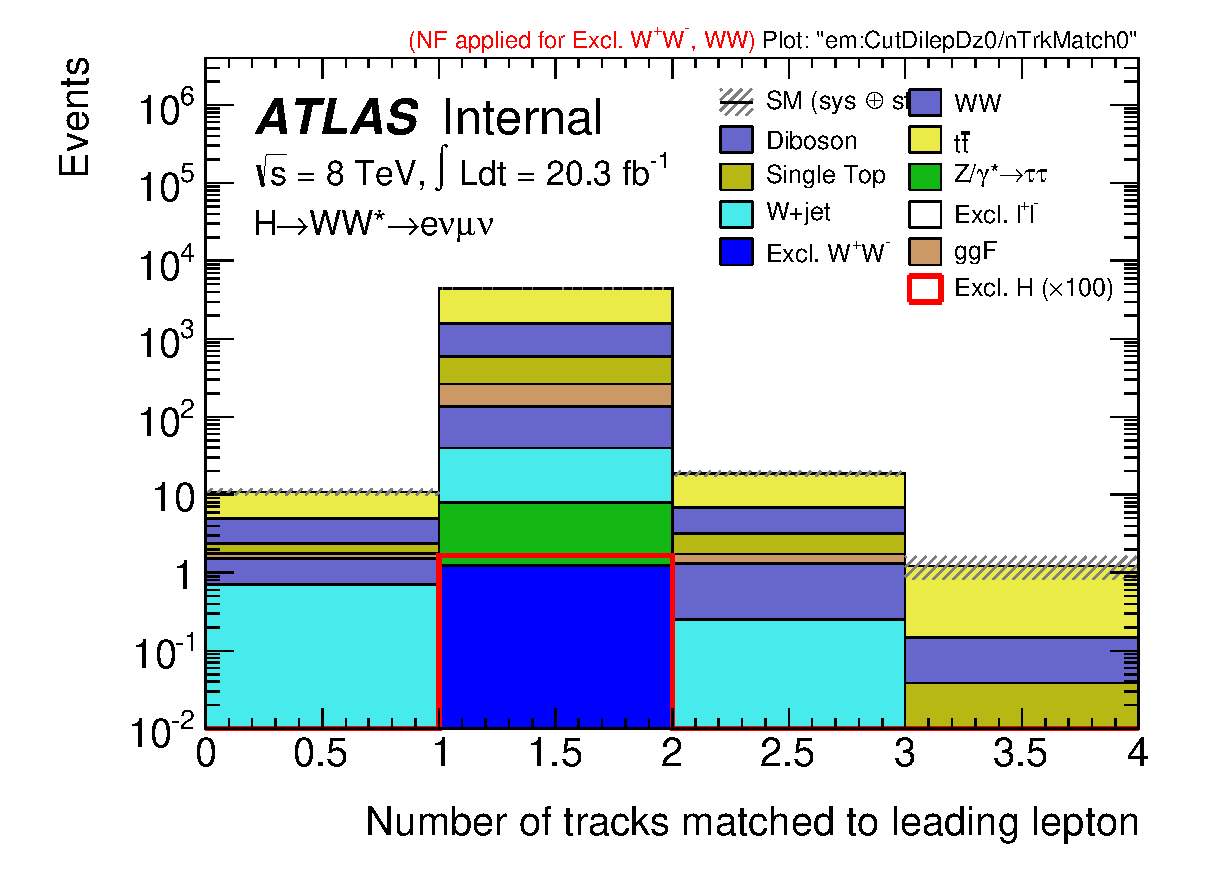
\includegraphics[width=0.5\linewidth]{em_CutDilepDz0_nTrkMatch0_mh125_log.eps}
	\includegraphics[width=0.5\linewidth]{me_CutDilepDz0_nTrkMatch0_mh125_log.eps}\\
\end{tabular}
\caption{Number of tracks from the trk container that are matched to the leading 
lepton tracks. [Left] The leading lepton is an electron. [Right] The leading lepton 
is a muon.}
\label{fig:trackMatching}
\end{figure}

\par Because electrons undergo bremsstrahlung more frequently than muons, there are more tracks 
matched to electrons than to muons. All the tracks matched to a lepton are therefore 
considered to be brehming from that lepton.

\par The exclusivity cut depends on how far in \z0\ the closest unmatched track 
is from the lepton track pair. Figure~\ref{fig:cartoon} illustrates how this is quantified. 
The two lepton tracks are first required to be within 1 mm in \z0\ to ensure that they indeed 
are from the lepton pair. The average \z0\ position computed from the individual lepton track \z0's is 
considered the dilepton vertex. The distance of the closest unmatched track $\Delta z_1$ is the 
exclusivity variable that is cut on. Figure~\ref{fig:deltaZ1} shows $\Delta z_1$  for signal and several backgrounds.
The signal is scaled by a factor of 100 to make it visible because it is heavily dominated by the backgrounds.
The $\Delta z_1$ distribution in signal and other exclusive processes 
is characterized by a tail more spread out than in inclusive processes. Several values of $\Delta z_1$ 
were tried to maximize $signal/\sqrt{background}$. Figure~\ref{fig:sOverB} shows $signal/\sqrt{background}$
for four values of $\Delta z_1$. This analysis settles on $\Delta z_1 > 1 mm$ as the optimal 
exclusivity cut.    

\begin{figure}[t]
\centering
\includegraphics[width=0.4\linewidth]{cartoon.eps}
\caption{Illustration of the exclusivity variables.}
\label{fig:cartoon}
\end{figure}

\begin{figure}[!h]
\centering
\begin{tabular}{c}
	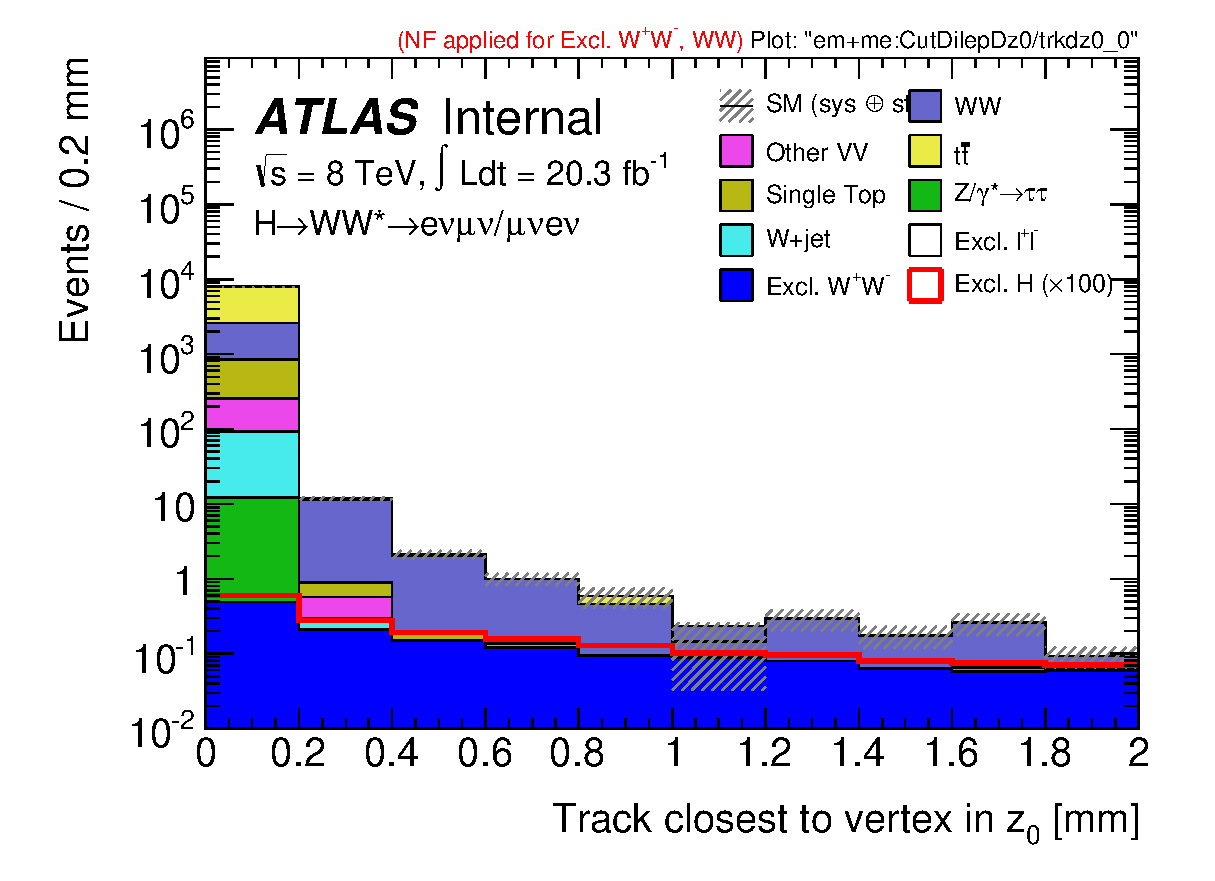
\includegraphics[width=0.5\linewidth]{trkdz0_deltaZ1.eps}
\end{tabular}
\caption{The main exclusivity variable $\Delta z_1$, which is the distance of 
the closest unmatched track to the dilepton vertex in \z0. Signal is scaled by 100. 
$\Delta z_1$ has a longer tail in exclusive processes compared to inclusive processes. 
This distrinction is exploited in this study.}
\label{fig:deltaZ1}
\end{figure}

\begin{figure}[!h]
\centering
\begin{tabular}{c}
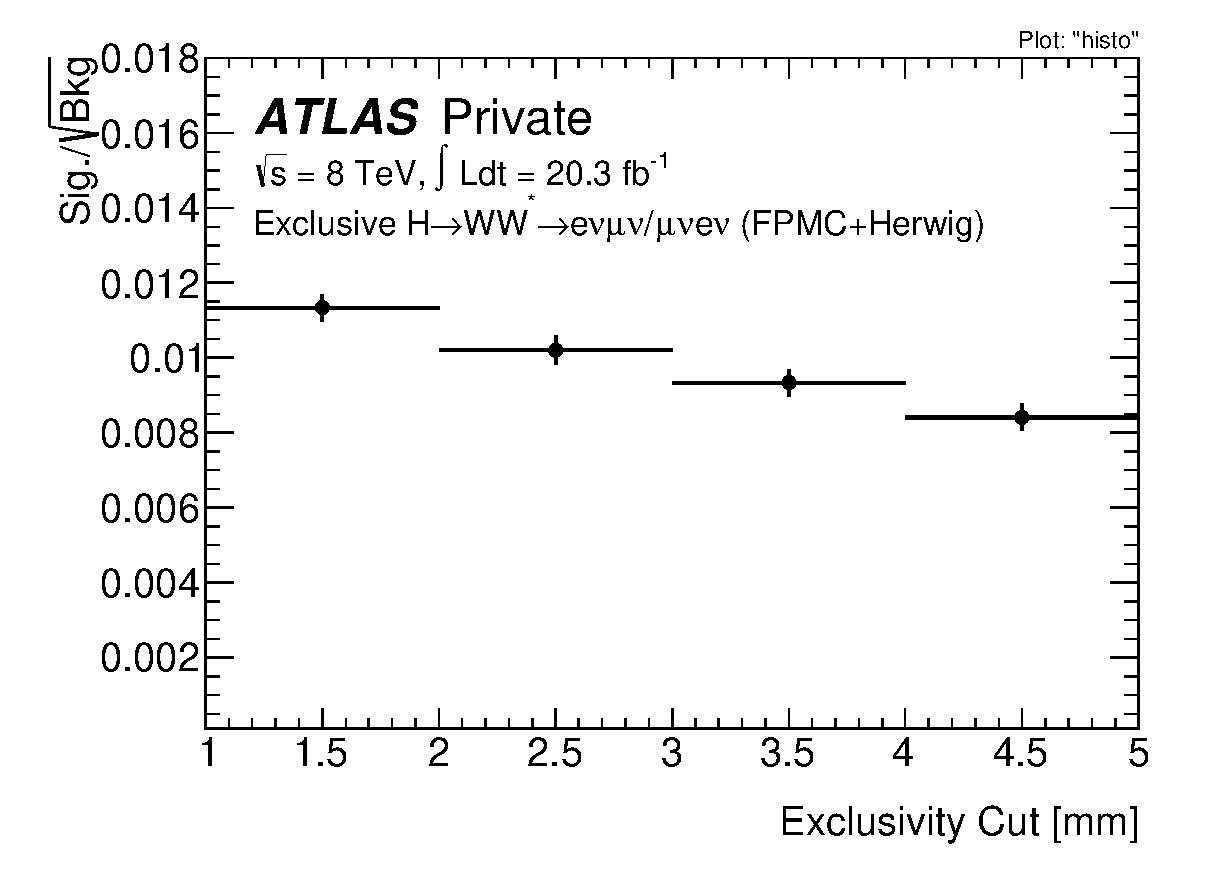
\includegraphics[width=0.7\linewidth]{emme_sOverB.eps}
\end{tabular}
\caption{$signal/\sqrt{background}$ for 4 values of $\Delta z_1$. This analysis settles 
on $\Delta z_1 > 1 mm$ as the optimal exclusivity cut.}
\label{fig:sOverB}
\end{figure}

\subsection{Performance in data}
\par A region in data that is rich in \Ztau\ events is used to validate the exclusivity selection 
criteria. This region follows the control region used in Ref.~\cite{ATLASCONF2014060} to constrain 
 \Ztau+0-jets events in the \HWW\ study. In this study we apply it to any jet multiplicity.
The selection is similar to the signal selection criteria except the following: \mll\ region is expanded to 
cover $10<\mll<80 $GeV, \ptll\ is changed to $\ptll<30 $GeV. There is no \dfll\ cut. Figure~\ref{fig:ztauCR}
shows some kinematic distributions of events in this \Ztau\ region. Before exclusivity, MC over-estimate 
\Ztau\ yields by 0.3\% in this region. After exclusivity MC over-estimate the yield by 387\%.
This is because MC mismodeles the underlying event. Table~\ref{table:ztauCR} shows the event yields in both
data and MC. Figure~\ref{fig:ztauCR} shows key kinematic distributions before exclusivity is imposed 
in this control region. The good agreement between data and MC testify to the purity of the \Ztau\ events
in data.  

\begin{table}
\centering
        \resizebox{.6\textwidth}{!}{
\begin{tabular}{l||r|rr}
 & $Z+\gamma/$jets & Observed & Data/MC \\
\hline\hline
blinding & 34360.39 $\pm$ 473.93 & 92352 & 1.19 $\pm$ 0.01 \\
lepton $p_{\mathrm{T}}$ & 17990.93 $\pm$ 346.30 & 62517 & 1.12 $\pm$ 0.01 \\
OS leptons & 17821.85 $\pm$ 344.56 & 60072 & 1.10 $\pm$ 0.01 \\
$m_{\ell\ell} > 10$ GeV & 17803.29 $\pm$ 344.32 & 60002 & 1.10 $\pm$ 0.01 \\
$E^{\mathrm{miss}}_{\mathrm{T,rel}} < 25$ GeV & 13722.36 $\pm$ 300.23 & 28896 & 1.08 $\pm$ 0.01 \\
$\Delta\phi_{\ell\ell, MET} > 1.57$ & 11127.20 $\pm$ 270.22 & 19390 & 1.04 $\pm$ 0.02 \\
$p_{\mathrm{T},\ell\ell}<$30 GeV & 10908.72 $\pm$ 267.29 & 12060 & 0.98 $\pm$ 0.02 \\
$m_{\ell\ell}<80$ GeV & 10651.88 $\pm$ 264.46 & 10600 & 0.95 $\pm$ 0.02 \\
$\Delta z^{0}_{ll}<1.0$ mm & 10576.86 $\pm$ 263.56 & 10538 & 0.95 $\pm$ 0.02 \\
\hline
1 mm Exclusive & 58.38 $\pm$ 19.86 & 12 & 0.21 $\pm$ 0.09 \\
\end{tabular}
}
\label{table:ztauCR}
\caption{\Ztau\ yields in the \Ztau\ control region. Right before exclusivity is imposed, MC over-estimate 
\Ztau\ yields by 0.3\%. After exclusivity, the over-estimation rises to 387\%.}
\end{table}


\begin{figure}[!h]
\centering
\begin{tabular}{c}
	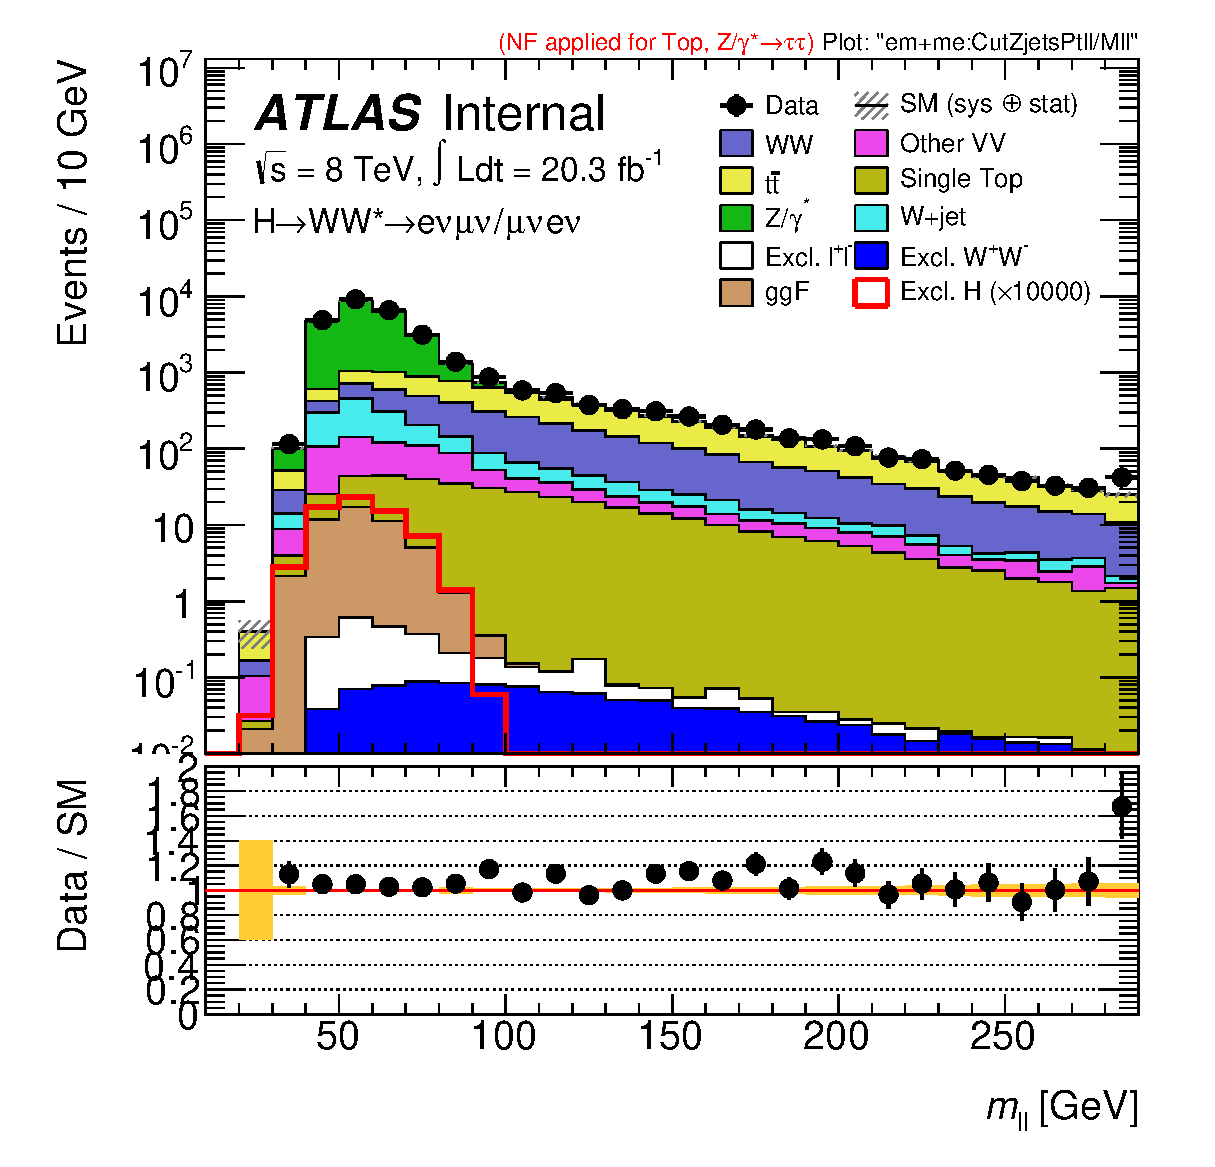
\includegraphics[width=0.5\linewidth]{emme_CutZjetsPtll_Mll_mh125_log.eps}
	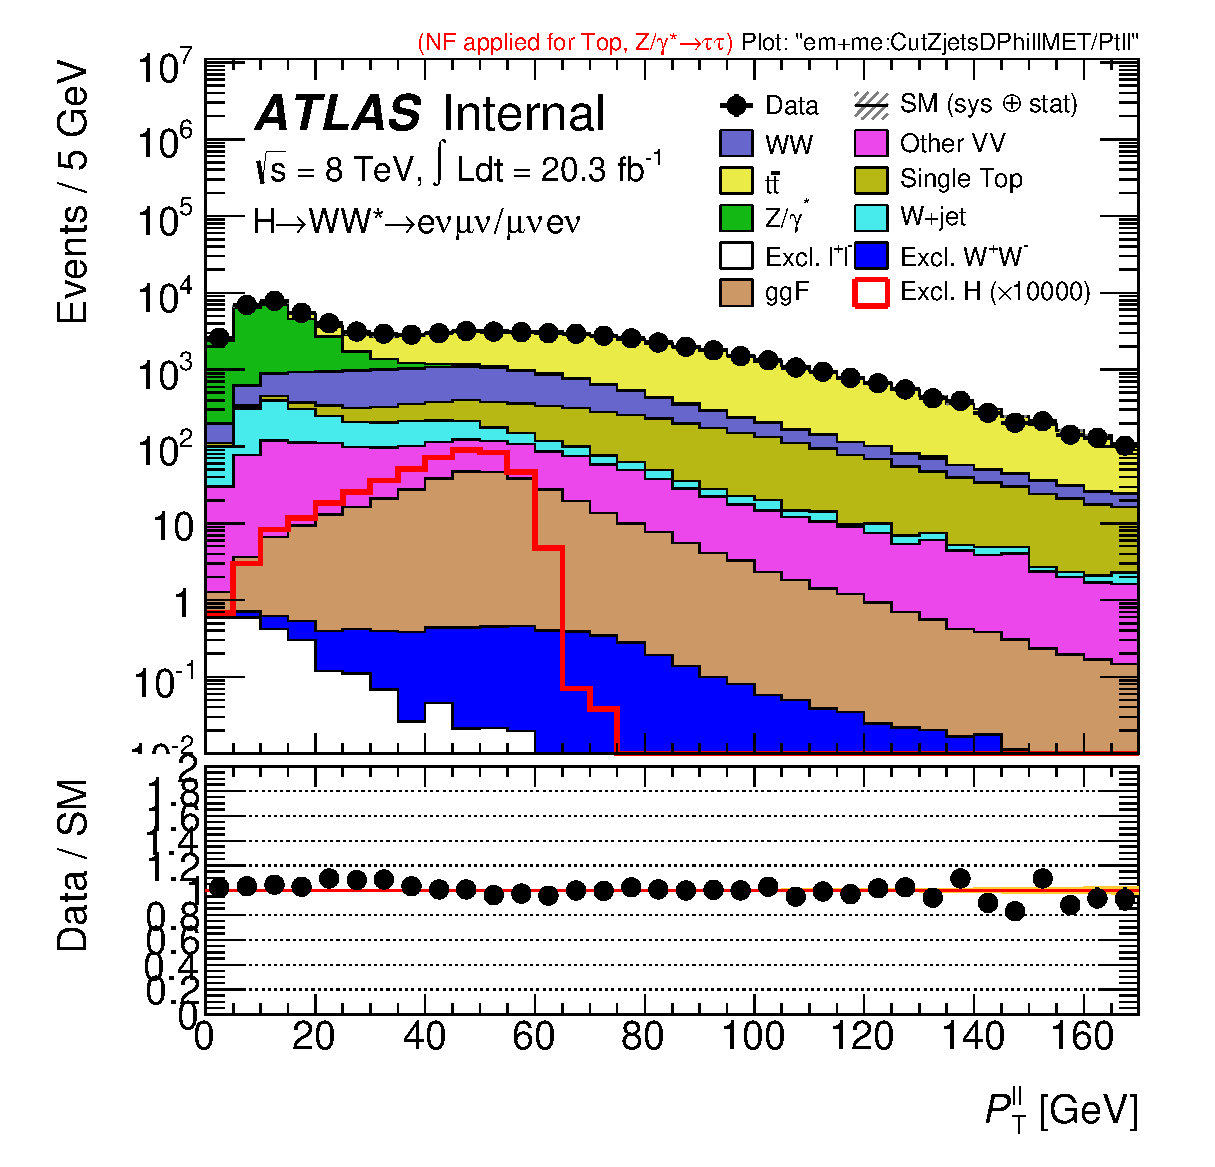
\includegraphics[width=0.5\linewidth]{emme_CutZjetsDPhillMET_Ptll_mh125_log.eps}\\
	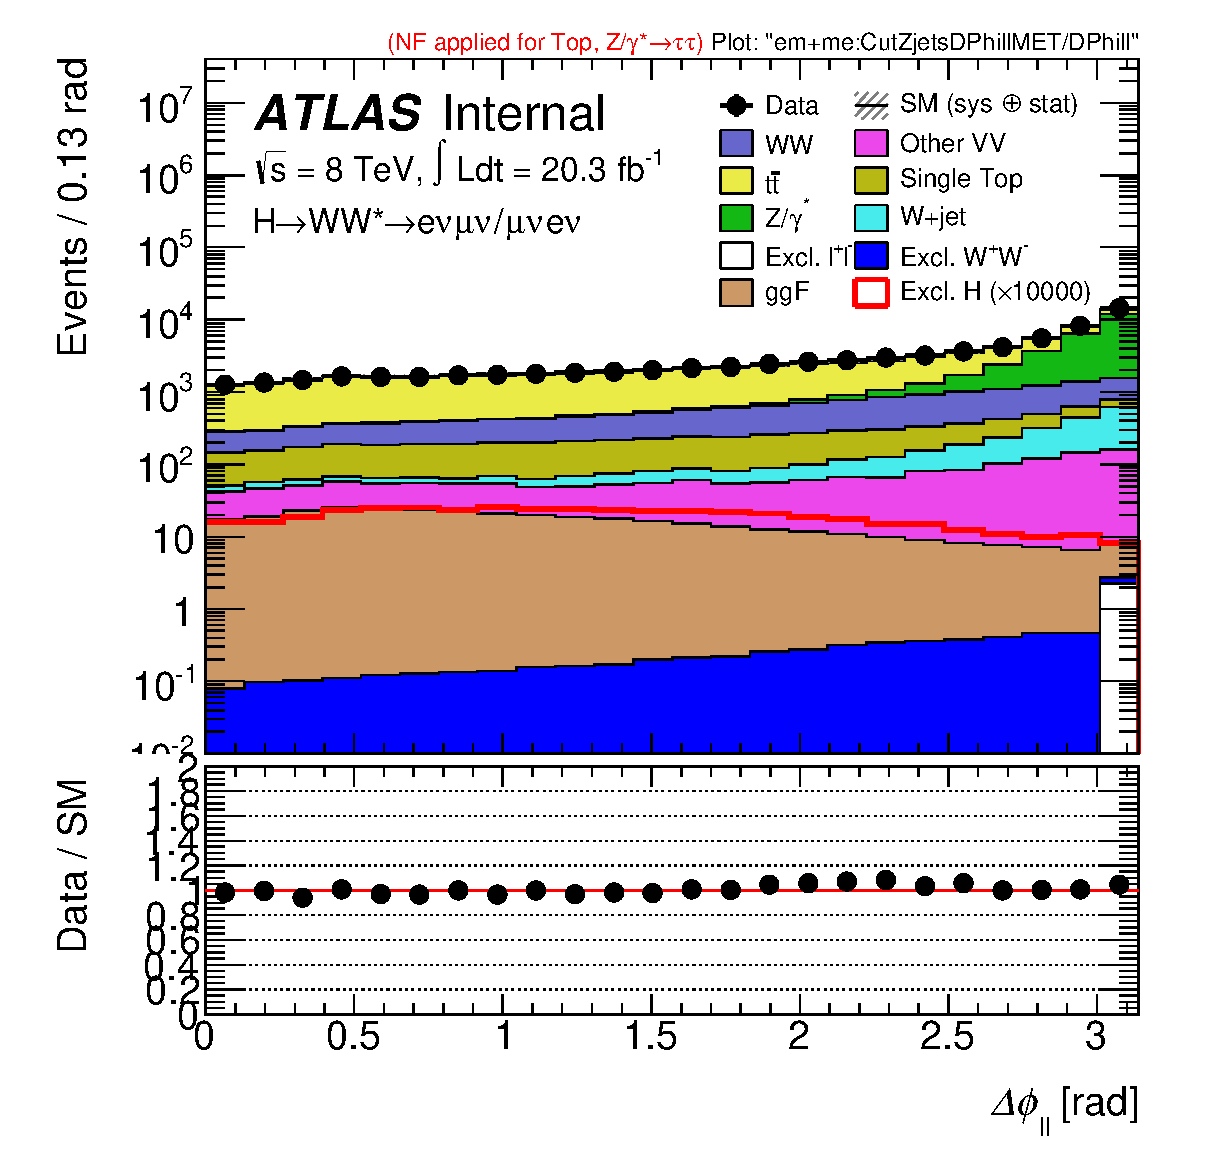
\includegraphics[width=0.5\linewidth]{emme_CutZjetsDPhillMET_DPhill_mh125_log.eps}
	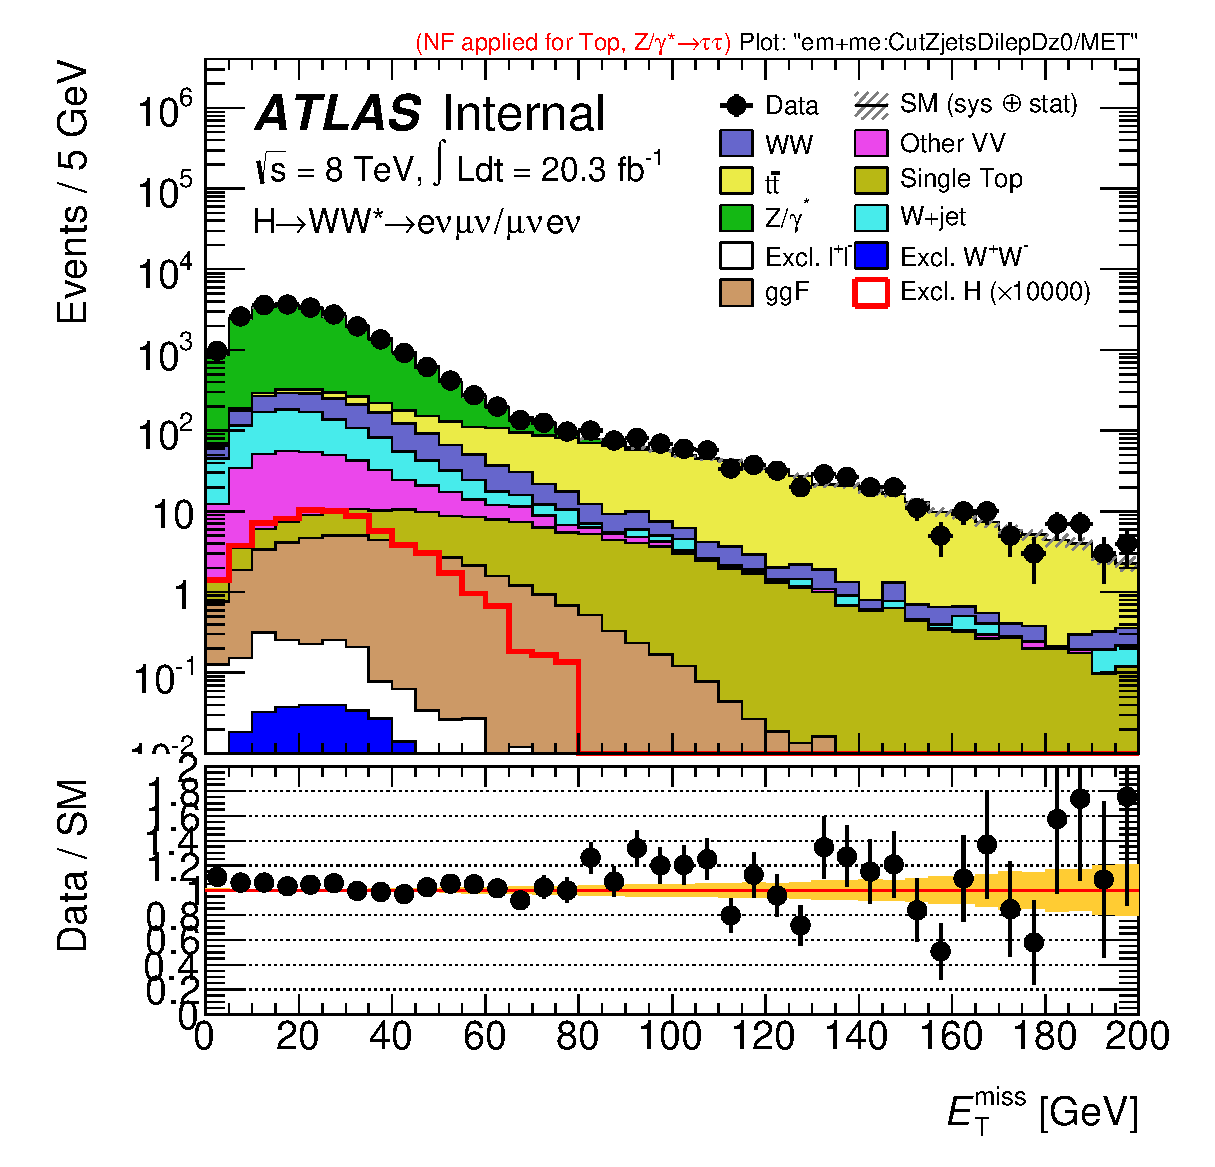
\includegraphics[width=0.5\linewidth]{emme_CutZjetsDilepDz0_MET_mh125_log.eps}\\
	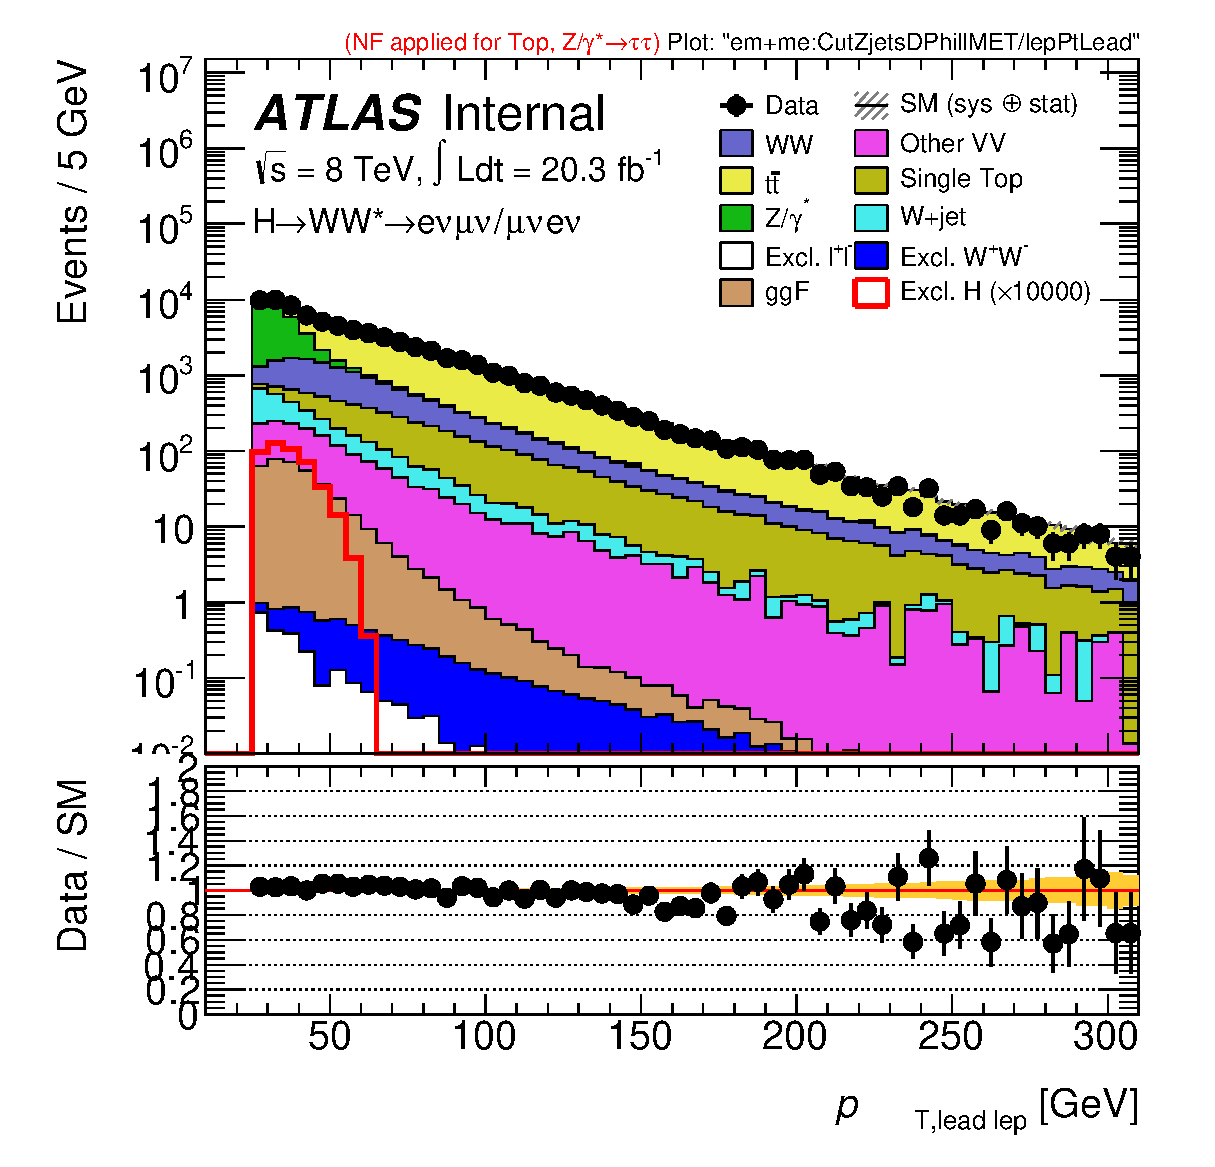
\includegraphics[width=0.5\linewidth]{emme_CutZjetsDPhillMET_lepPtLead_mh125_log.eps}
	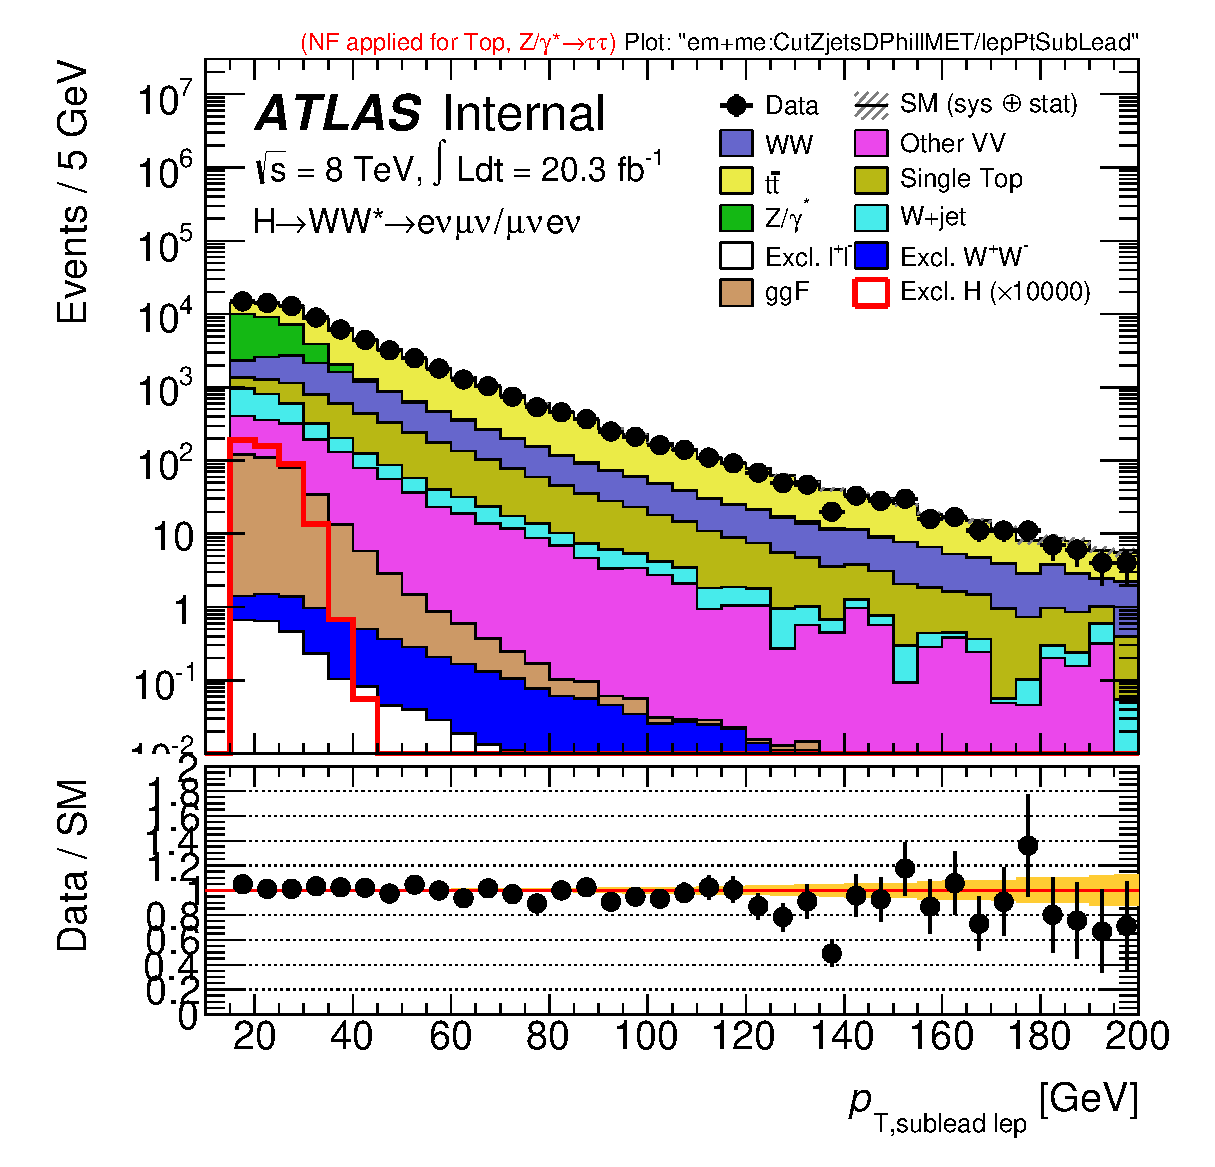
\includegraphics[width=0.5\linewidth]{emme_CutZjetsDPhillMET_lepPtSubLead_mh125_log.eps}\\
\end{tabular}
\caption{Key kinematic distributions in the \Ztau\ control region before the exclusivity cut is imposed.}
\label{fig:ztauCR}
\end{figure}

\par Figure~\ref{figztauExclCR} shows distributions for exclusivity variables before the exclusivity cut is imposed.
The difference in $z_0$ between the two lepton tracks is also affected by the underlying event. The $\Delta z_1$
distribution shows a uniform disagreement between data and MC for $\Delta z_1>1$ mm. This disagreement results in the 
387\% data/MC disagreement alluded to in the preceding paragraph. To correct for this we introduce  a correction factor, 

\begin{equation}
\mbox{MC Exclusivity Correction Factor, MF} = \frac{N^{mc}_{after\ excl.}/N^{mc}_{before\ excl.}}{N^{data}_{after\ excl.}/N^{data}_{before\ excl.}}
\end{equation}

which is the ratio of the exclusivity cut efficiency in MC to its efficiency in data.
Ideally it is 1.0 if MC models the underlying event correctly. An MF larger than 1.0 implies that MC over-estimate
events that pass the exclusivity cut. The Alpgen+Jimmy MC that we use for this region give $MF=4.72$. 
 
\begin{figure}[!h]
\centering
\begin{tabular}{c}
	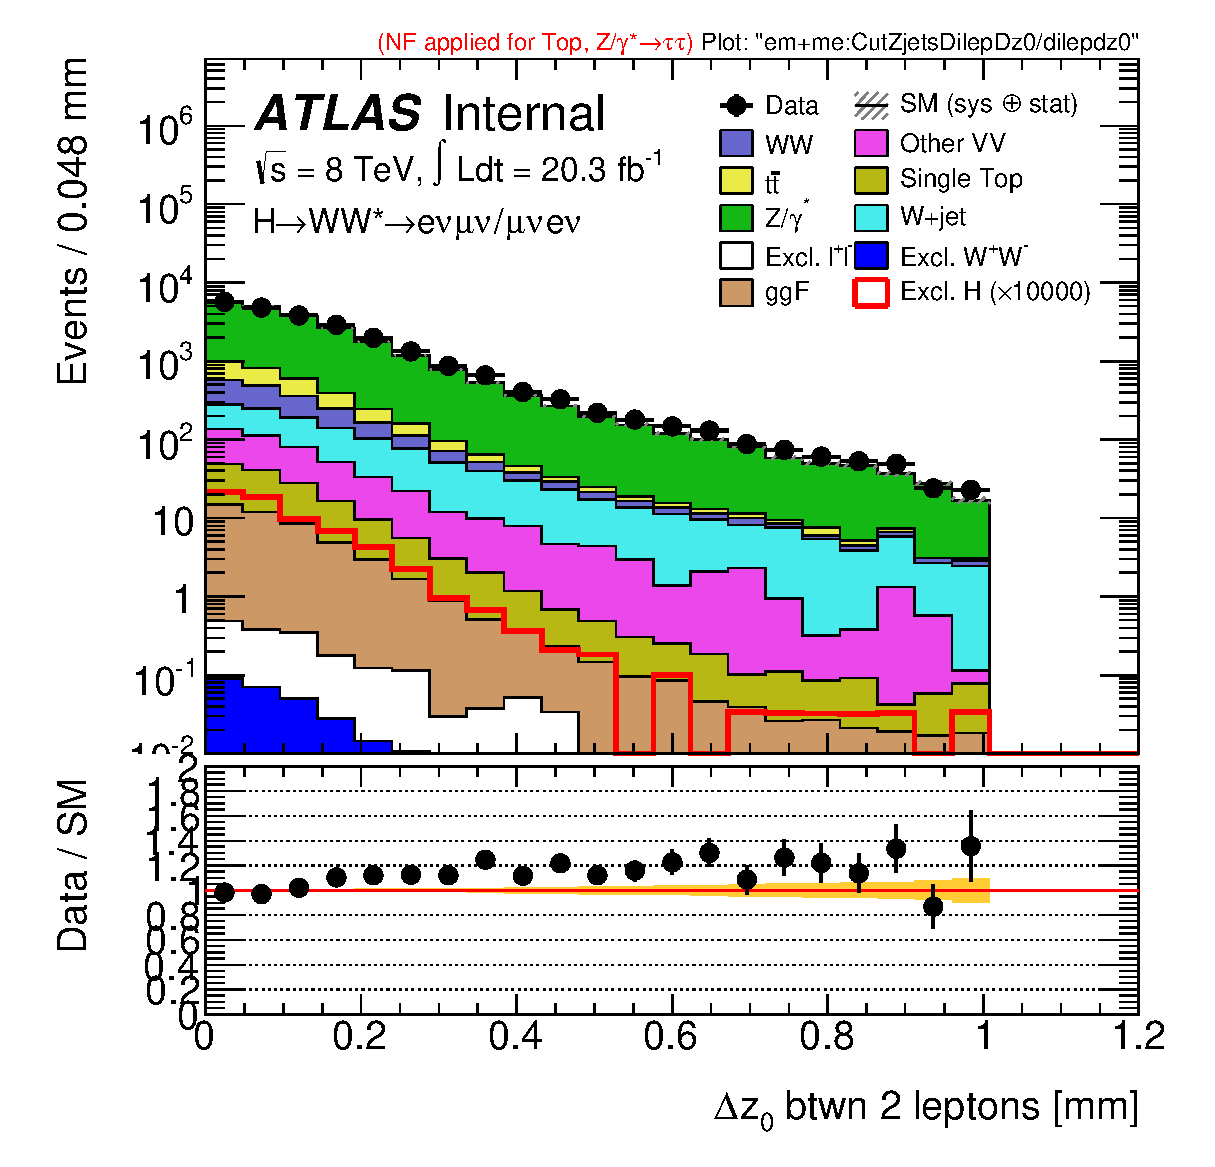
\includegraphics[width=0.5\linewidth]{emme_CutZjetsDilepDz0_dilepdz0_mh125_log.eps}
	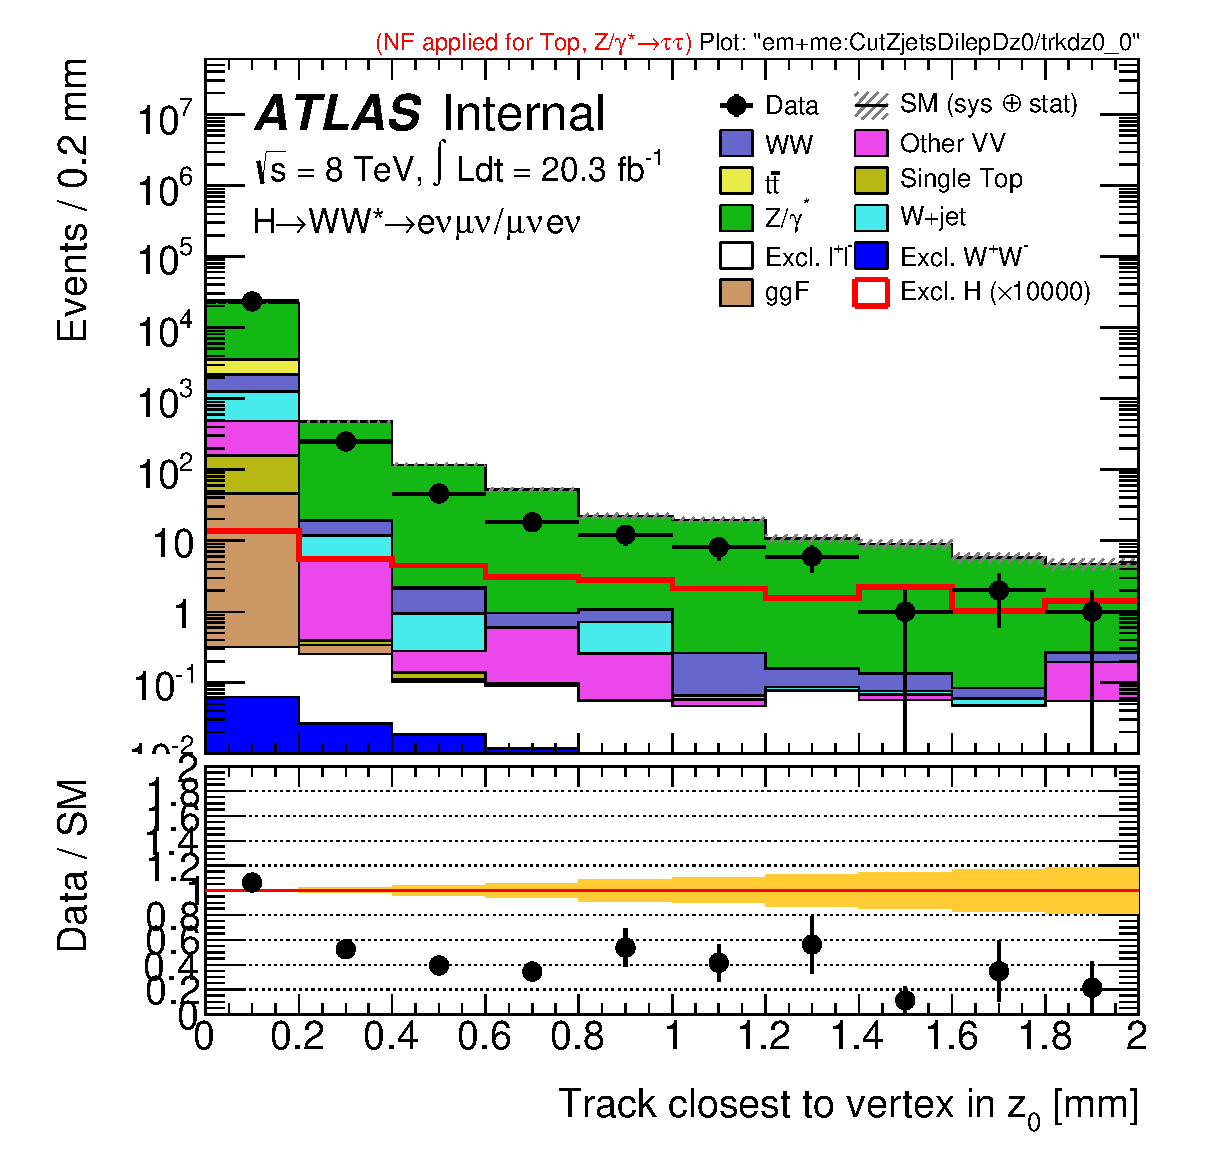
\includegraphics[width=0.5\linewidth]{emme_CutZjetsDilepDz0_trkdz0_0_mh125_log.eps}\\
\end{tabular}
\caption{Exclusivity variables in the \Ztau\ control region show a disagreement between data and MC. This
motivates the use of a correction factor on the MC.}
\label{fig:ztauExclCR}
\end{figure}

\par Studies similar to the \Ztau\ study were done using \Zmm\ events, estimating them 
with several MC listed in Table~\ref{table:mf}. The resulting MFs are listed in the same table.
All MC studied tend to over-estimate events that pass the exclusivity cut. Of all these MC,
Sherpa over-estimates the most. Figure~\ref{fig:mf} shows the number of tracks within a 1.0 mm
around the di-muon vertex, computed as shown in Figure~\ref{fig:cartoon}. The exclusivity cut select 
only the events that are in the first bin of these plots. Clearly Sherpa over-estimates these 
events by a factor close to 10 (9.23 to be precise). Because this analysis relies heavily on 
MC to estimate major backgrounds, it is necessary to correct the MC using MFs. By comparing the 
Alpgen+Jimmy MF obtained using \Zmm\ events to the one obtained using \Ztau\ events we notice 
that they agree within 8\%. Clearly the MF is a major source of systematic uncertainties. We will 
discuss these in Section~\ref{sec:syst}.  

\begin{table}
\begin{center}
        \resizebox{0.4\textwidth}{!}{
\providecommand{\cutflowTitle}{hsg3}
\begin{tabular}{l|rr}
 & \Zmm & \Ztau   \\
\hline\hline
Sherpa &       9.23 &  \\
AlpgenPythia & 1.65 & \\
AlpgenJimmy & 4.36  & 4.72\\
PowhegPythia & 2.35 & 
\end{tabular}
}
\caption{MFs obtained from studying \Zmm\ and \Ztau\ events and estimating them using several MC. Sherpa 
mismodels the underlying event the worst. We use Alpgen+Jimmy MC in this analysis.}
\label{table:mf}
\end{center}
\end{table}

\begin{figure}[!h]
\begin{tabular}{c}
	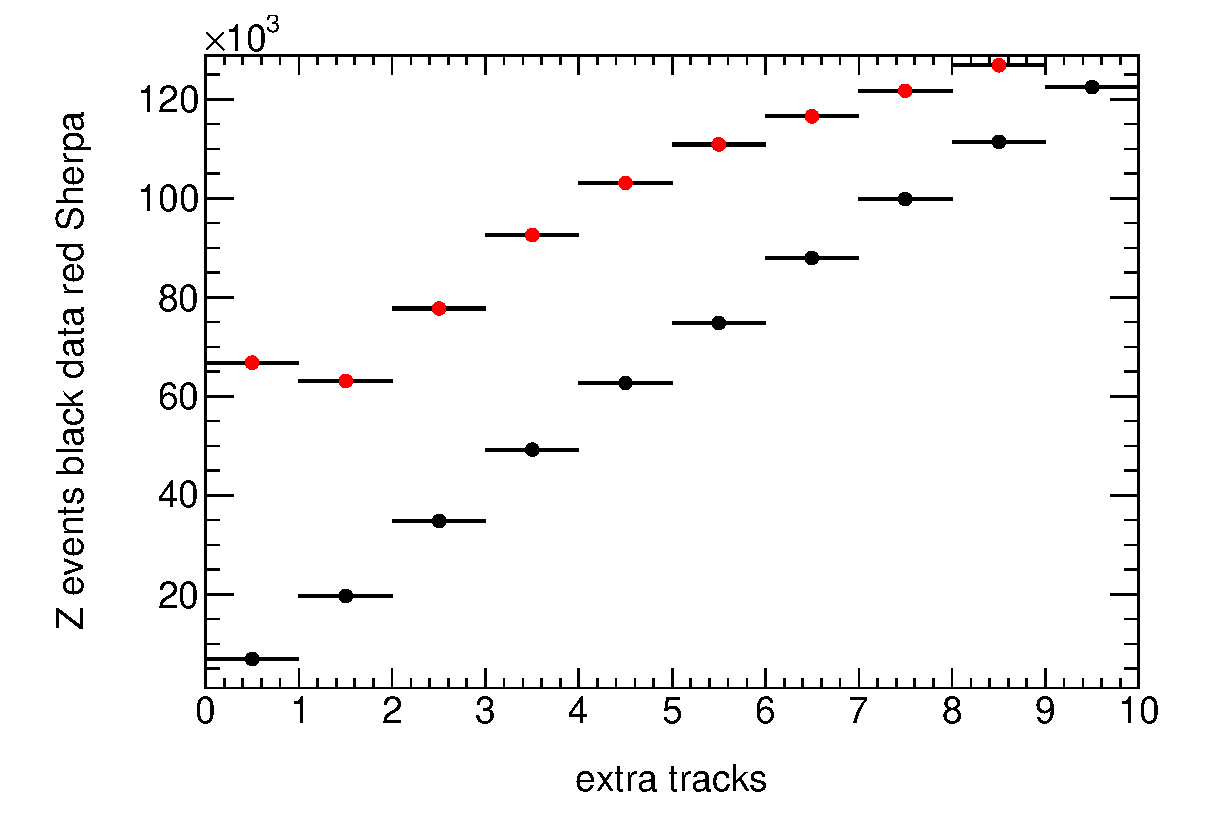
\includegraphics[width=0.5\linewidth]{extraZsherpa.eps}
	\includegraphics[width=0.5\linewidth]{extraZpowheg.eps}
\end{tabular}
\caption{Number of extra tracks within a 1.0 mm window around the di-muon vertex calculated as 
shown in Figure~\ref{fig:cartoon}. Events that pass exclusivity cut are in the first bin of these plots.
Sherpa clearly is the worst at modelling the underlying event. }
\label{fig:mf}
\end{figure}
